\chapter{Iteración 6}

\begin{quotation}[Software Engineer]{Martin Fowler (1963--)}
Any fool can write code that a computer can understand. Good programmers write code that humans can understand.
\end{quotation}

\begin{abstract}
Esta iteración introduce sistemas de soporte que amplían la profundidad de la partida. El
trabajo se centra en la gestión del inventario, la incorporación de objetos interactivos y
la evolución del minimapa, preparando una experiencia más completa y mejor estructurada.
\end{abstract}

\section{Análisis de características}
La sexta iteración se centró en incorporar una primera capa real de progresión basada en
objetos y en consolidar una segunda mejora del minimapa. Hasta este momento, el jugador ya
podía explorar, combatir y progresar entre círculos, pero todavía no disponía de un sistema
interno de inventario capaz de almacenar recompensas, seleccionar contenido adquirido o
relacionar el mundo con objetos persistentes de la partida. Por ello, esta iteración se
estructura en torno a tres funcionalidades: la gestión de inventario, los objetos y una
segunda mejora del minimapa orientada a convertirlo en un apoyo de navegación más claro,
reactivo y coherente con el estado real de la mazmorra.

\begin{enumerate}
\item \textbf{Gestión de Inventario.} Esta funcionalidad introdujo la base runtime del
inventario del jugador, organizando la colección de objetos en una estructura de slots con
capacidad limitada y con selección activa. Su funcionamiento real se apoya en un inventario
de doce posiciones potenciales, aunque no todas están desbloqueadas desde el comienzo, lo
que permite tratar la capacidad como parte de la progresión del personaje. La feature
incorpora operaciones para seleccionar slots, añadir objetos válidos, soltar el objeto del
slot actual y notificar a la interfaz cuando se produce un cambio. También contempla casos
de error como inventario lleno, slot vacío, slot bloqueado u objeto inválido, registrando
la causa del fallo para facilitar la comunicación con el jugador o con herramientas de
depuración. En términos funcionales, esta feature convierte la acumulación de objetos en una
parte real del sistema, ya que deja de tratarse de elementos efímeros en el mundo y pasa a
existir una estructura persistente de almacenamiento asociada al jugador.

\begin{figure}[H]
\begin{center}
\missingfigure{Sustituir por captura representativa de Gestión de Inventario en la iteración 6}
% \includegraphics[width=.9\textwidth]{figures/iteracion6_gestion_inventario.png}
\caption{Resultado visual de la feature Gestión de Inventario en la iteración 6}
\label{fig:iteracion6-feature-inventario}
\end{center}
\end{figure}

\item \textbf{Objetos.} Esta funcionalidad definió la representación de los objetos como
entidades consistentes tanto en datos como en mundo. Su funcionamiento real se articula en
dos niveles. El primero es la definición del objeto como recurso configurable, con
identificador normalizado, nombre visible, icono, tipo y parámetros asociados a su efecto.
El segundo es su presencia dentro del mundo mediante pickups capaces de mostrar ese objeto,
permitir su recogida por parte del jugador y desaparecer cuando la operación tiene éxito.
La feature contempla además la validación de definiciones para evitar inconsistencias en los
datos y fuerza un modelo de objetos únicos no apilables, simplificando la lógica inicial del
inventario. En conjunto, esta funcionalidad conecta por primera vez el contenido recogible
del escenario con una representación interna estructurada y con la interfaz del inventario,
haciendo posible que los objetos se conviertan en una unidad real de progresión jugable.

\begin{figure}[H]
\begin{center}
\missingfigure{Sustituir por captura representativa de Objetos en la iteración 6}
% \includegraphics[width=.9\textwidth]{figures/iteracion6_objetos.png}
\caption{Resultado visual de la feature Objetos en la iteración 6}
\label{fig:iteracion6-feature-objetos}
\end{center}
\end{figure}

\item \textbf{Minimap.} Esta funcionalidad completó una segunda mejora del minimapa sobre la
base ya introducida anteriormente. Su alcance real consistió en hacer que la representación
del mapa respondiera al progreso del jugador dentro de la partida, diferenciando entre salas
no descubiertas, salas visitadas y sala actual. Además, el sistema pasó a centrar la cámara
del minimapa sobre la habitación en la que se encuentra el jugador y a adaptar su
presentación visual al tamaño de pantalla mediante un contenedor con máscara, marco y fondo
propios. En términos funcionales, esta ampliación convirtió el minimapa en una herramienta
de orientación más legible, capaz de reflejar tanto el recorrido realizado como la posición
actual dentro de la mazmorra sin mostrar desde el principio toda la estructura del nivel.

\begin{figure}[H]
\begin{center}
\missingfigure{Sustituir por captura representativa de Minimap en la iteración 6}
% \includegraphics[width=.9\textwidth]{figures/iteracion6_minimap.png}
\caption{Resultado visual de la feature Minimap en la iteración 6}
\label{fig:iteracion6-feature-minimap}
\end{center}
\end{figure}
\end{enumerate}

La combinación de estas tres funcionalidades hace que la sexta iteración actúe como puente
entre el núcleo de combate ya consolidado y una capa de progresión más tangible basada en
recompensas, recogida de contenido y lectura más rica del estado de la partida.

\section{Diseño}
El diseño de esta iteración giró en torno a una idea central: convertir los objetos en
elementos persistentes y gestionables, en lugar de tratarlos como contenido aislado dentro
del mundo. Para ello era necesario definir una estructura interna de inventario, un formato
estable para los objetos y una forma clara de relacionar ambos sistemas con el jugador y con
la interfaz.

\subsection{Diseño de la gestión de inventario}
La principal decisión de diseño fue modelar el inventario como una colección cerrada de
slots, no como una lista ilimitada de entradas dinámicas. Esto facilita el control del HUD,
la selección activa y la idea de capacidad desbloqueable como parte de la progresión del
personaje.

Además, se decidió separar la lógica de selección, la lógica de almacenamiento y la gestión
de errores, de modo que el sistema pueda reaccionar de forma distinta según la operación que
falle. La presencia de slots bloqueados desde el diseño también prepara el terreno para
mejoras futuras sin obligar a rediseñar el modelo base del inventario.

\subsection{Diseño de los objetos}
Los objetos se diseñaron como definiciones de datos independientes del pickup físico que los
representa en el mundo. Esta separación era importante porque evita mezclar configuración y
representación visual, permitiendo que un mismo tipo de objeto pueda existir como recurso
abstracto, como icono de inventario o como entidad recogible.

También se tomó la decisión de imponer, en esta primera fase, una política de objetos
únicos no apilables. Esto reduce la complejidad inicial del sistema y hace que cada slot
tenga una interpretación directa, algo útil mientras el inventario aún se encuentra en una
fase relativamente temprana.

\subsection{Diseño de la ampliación del minimapa}
La segunda fase del minimapa se diseñó alrededor de una idea sencilla: la información del
mapa debía revelarse en función del recorrido real del jugador, no mostrarse completa desde
el inicio. Para ello se optó por separar tres estados visuales distintos, correspondientes a
salas ocultas, salas ya visitadas y sala actual, de modo que el minimapa funcionara también
como resumen del progreso de exploración.

Además, se decidió desacoplar la lógica de descubrimiento, el centrado de cámara y la
presentación en interfaz. Esta separación permite que el estado de las salas quede
gestionado por el generador del mapa, mientras que la cámara del minimapa y su contenedor de
interfaz puedan evolucionar sin depender de cambios estructurales sobre la lógica de
generación.

\section{Implementación}
La implementación de esta iteración se apoyó sobre todo en la incorporación de nuevos tipos
de dato y en la conexión entre mundo, jugador e interfaz. A diferencia de la iteración
anterior, donde el foco estaba claramente en combate y enemigos, aquí el peso recae en la
gestión del contenido recogible y en su persistencia durante la partida.

\subsection{Implementación de la gestión de inventario}
La lógica principal quedó centralizada en \texttt{PlayerInventory}. Este componente
implementa un inventario de tamaño máximo fijo, mantiene el índice del slot seleccionado y
expone operaciones para cambiar de slot, añadir objetos y soltar el objeto activo. También
se apoya en eventos para notificar modificaciones, lo que permite desacoplar la actualización
del inventario de su representación visual en la interfaz.

La capacidad disponible se enlaza con \texttt{PlayerStats}, de forma que el número de slots
desbloqueados puede depender del estado de progresión del jugador. A ello se suma una lógica
de validación de operaciones que registra por qué una acción falla, lo que resulta útil
tanto para depuración como para la futura comunicación con el usuario.

\subsection{Implementación de los objetos}
La representación de los objetos se apoyó en \texttt{InventoryItemDefinition}, que define la
identidad del objeto, su icono, su tipo y los datos asociados a sus posibles efectos.
Además, \texttt{InventoryItemValidationUtility} se encarga de validar estas definiciones y
de normalizar identificadores para evitar inconsistencias.

La presencia física del objeto en el mundo se resolvió mediante \texttt{WorldInventoryPickup},
un componente encargado de mostrar el icono del ítem, ofrecer una operación de recogida
contra el inventario del jugador y destruir o mantener el pickup según el resultado. Esto
permite que el vínculo entre mundo e inventario quede resuelto de manera directa: el jugador
interactúa con un pickup y, si la operación es válida, el objeto pasa a su inventario.

\subsection{Implementación de la mejora del minimapa}
La ampliación del minimapa se apoyó principalmente en \texttt{MapGenerator},
\texttt{MinimapCameraController} y \texttt{MinimapUIController}. En primer lugar,
\texttt{MapGenerator} pasó a mantener el conjunto de salas visitadas, la sala actual y un
sistema de actualización visual basado en niveles de opacidad. Con ello, cada celda puede
representarse como no descubierta, visitada o activa, y el refresco del minimapa se produce
cuando el jugador entra en una nueva habitación.

En segundo lugar, \texttt{MinimapCameraController} se encarga de seguir la sala actual del
jugador, centrando la cámara del minimapa sobre la celda correspondiente en lugar de dejar
una vista fija de todo el nivel. Esto hace que la lectura del mapa se mantenga focalizada en
la zona relevante de la exploración.

Por último, \texttt{MinimapUIController} reorganiza la imagen del minimapa dentro del HUD,
creando un contenedor propio con máscara, fondo y marco, además de recalcular su tamaño y
su margen en función de la resolución disponible. De esta forma, la mejora no solo afecta al
contenido mostrado, sino también a la calidad de su integración visual en pantalla.

\section{Seguimiento y control}
El seguimiento de la iteración muestra la introducción de una base clara para la progresión
por objetos y una mejora tangible de la lectura del mapa. El jugador pasó a disponer de una
estructura de inventario real, el mundo pudo contener pickups conectados con ese inventario
y el minimapa dejó de ser una referencia estática para convertirse en una vista más útil del
recorrido y de la posición actual dentro de la partida.

De forma resumida, al final de esta iteración se había conseguido:

\begin{itemize}
    \item incorporar un inventario por slots con capacidad limitada y selección activa;
    \item definir objetos con identidad, icono, tipo y validación interna;
    \item conectar pickups del mundo con el inventario del jugador;
    \item preparar la progresión de capacidad del inventario desde las estadísticas del jugador;
    \item consolidar un minimapa con descubrimiento progresivo, resaltado de sala actual y adaptación al HUD.
\end{itemize}

Desde el punto de vista del control del desarrollo, esta iteración fue importante porque añadió
una capa de persistencia y recompensa que el proyecto todavía no tenía de forma clara, al
tiempo que mejoró la navegación momentánea dentro de cada \textit{run}. A partir de aquí,
los objetos pueden empezar a desempeñar un papel más fuerte en la economía y la progresión,
y el minimapa queda preparado para convivir con una estructura de salas cada vez más rica.
No se aprecia una desviación grave, aunque la iteración deja trabajo preparado para cierres
posteriores de balance y contenido.

\begin{table}[h!]
    \centering
    \begin{coolTable}{lr}{2}
    {Horas de la iteración 6}
    \textbf{Horas planificadas de la iteración} & 50:00 \\
    \textbf{Horas reales (Adolfo Borrego González)} & 26:39 \\
    \textbf{Horas reales (Germán Sánchez Carmona)} & 22:48 \\
    \textbf{Horas reales totales de la iteración} & 49:27 \\
    \textbf{Horas acumuladas planificadas hasta esta iteración} & 400:00 \\
    \textbf{Horas acumuladas reales hasta esta iteración} & 401:19 \\
    \end{coolTable}
    \caption{Resumen de horas reales de la iteración 6.}
\end{table}

\begin{figure}[htbp]
\begin{center}
% \missingfigure{Sustituir por el diagrama UML de resultado de la iteración 6}
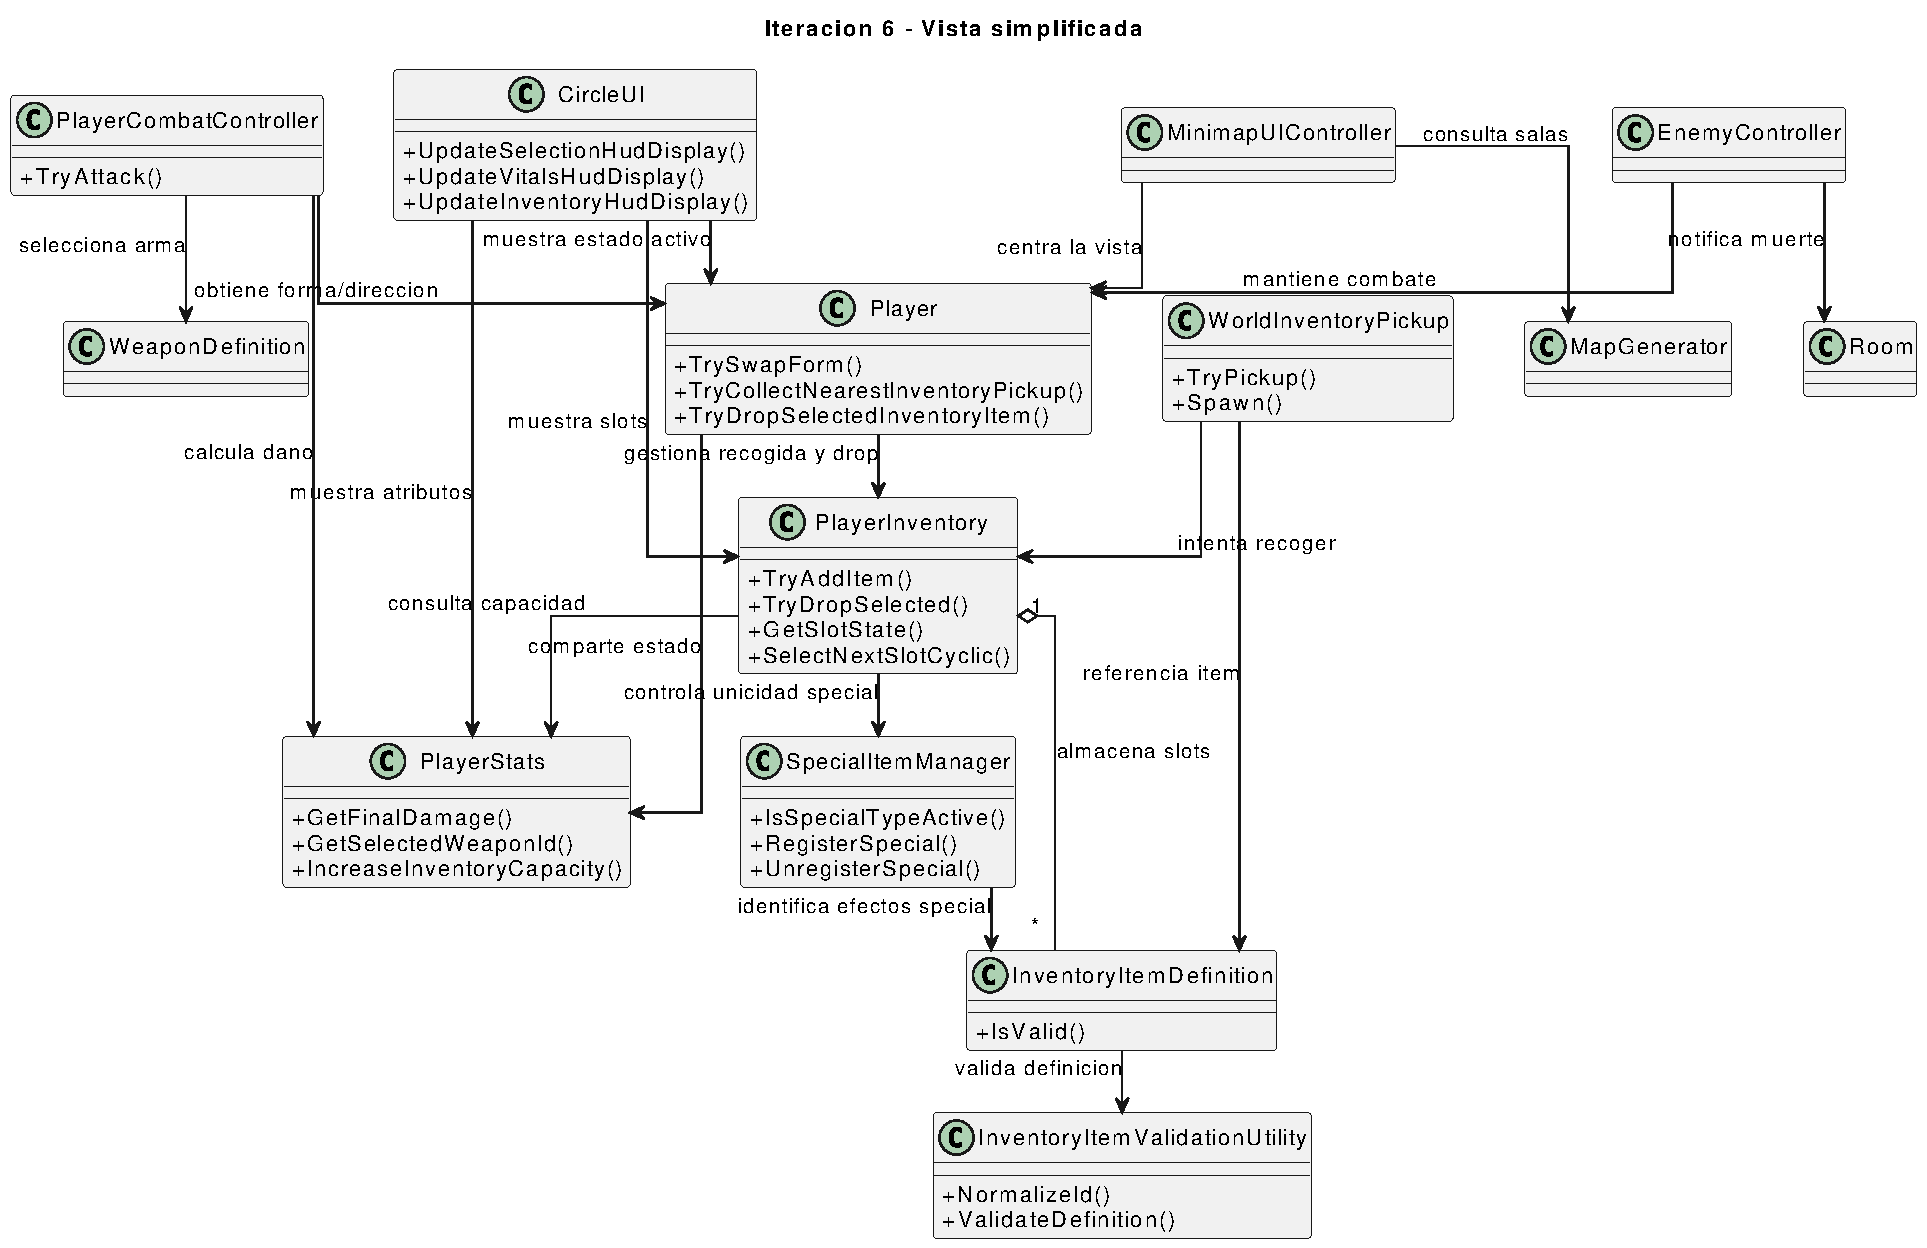
\includegraphics[width=\textwidth]{figures/iteracion6_resultado_uml.pdf}
\caption{Diagrama UML de resultado de la iteración 6}
\label{fig:uml-resultado-iteracion6}
\end{center}
\end{figure}
